\chapter{Optimized weights for the horizontal collaborative SOM algorithm}

\minitoc{}
\newpage

\section{Introduction}

In this chapter, we present an optimization method for the case of horizontal collaborative clustering between SOM algorithms. Our method aims at answering several questions regarding the tuning of the collaborative parameters between local and collaborative terms when using topological based collaborative clustering methods. 

The contributions presented in this chapter are 3-folds:

\begin{itemize}
	\item We propose an entirely automated and unsupervised optimization method to adjust the strength of the collaboration between algorithms collaborating together via the SOM algorithm.
	\item We experimentally demonstrate that our optimization method can efficiently be used to detect noisy views that would otherwise deteriorate the quality of a collaboration between algorithms.
	\item We give the theoretical properties of our proposed model. In particular, we show that our optimization method results in applying a meta-clustering on the different views, thus grouping them according to their similarities. 
\end{itemize} 
To do so, we propose an optimization method of the collaborative process likelihood function using Karush-Kuhn-Tucker optimization~\cite{KKT1}, and we interpret the results found for the algorithms weights in term of how they evolve based on criterion such as the stability and diversity of the partitions. This work can be compared with earlier studies on the influence of quality and diversity in collaborative clustering~\cite{grozavu2011learning,DBLP:conf/ssci/RastinCGB15,DBLP:conf/ijcnn/GrozavuCB14,Sublime2017}. It is an improvement upon these works in the sense that we give a mathematical justification and the theoretical properties of our weighting method, and we remove an user input parameter from the optimization constraints~\cite{Sublime2017} which makes this chapter's results more generic. Furthermore, our experimental section goes deeper into the analysis of the effects of weighting views, and shows the ability of our method to detect noisy views.


The remainder of this chapter is organized as follows: Section~\ref{sec:opt-w} is devoted to the description of our proposed optimization method, as well as the interpretation of the proposed weights formulas, in Section~\ref{app:c}, some numerical experiments are proposed and analyzed. Finally, Section~\ref{sec:cc-conlu} presents a conclusion on the work presented in this chapter.

\label{sec:opt-w}

\section{Optimization problem}

In this chapter we  propose a different collaborative approach in which we modify the objective function~\eqref{eq:globalC} using a weighting  strategy to reduce the risk of negative collaboration: we study how the optimization of the weights of the combination function in Equation~\eqref{eq:globalC} can lead to an optimal value of the global function and reduce the risk of negative collaboration by further optimizing weight factors between the algorithms.

We begin by changing the values of the $\alpha$ by $\alpha_i=1$. We believe that it makes a lot more sense than the proposed square root which is never justified in the related works~\cite{grozavu2010topological,grozavu2011learning}. This helps us to properly evaluate the balance between the local and the collaborative term, for which 1 variable is enough.
We are therefore mainly interested in finding the positive weights $\beta^j_i$ that will determine the strength of the collaborative term. 
Moreover, as we restrict our study to the case of horizontal clustering, we would like to mention that in our theoretical model all data sets describe the same observations and all these collaborative data sets have the same number of observations but a different number of variables.  


For fixed local maps $w$, our strategy to minimize Equation~\eqref{eq:globalC} is to minimize the second term. Indeed, since the collaboration weights are only in the collaborative term and because the local likelihoods are fixed, we can ignore the local term in Equation~\eqref{eq:globalC}.

The minimization of the collaborative term is based on the dual form of the problem. We do so under the Karush-Kuhn-Tucker conditions (KKT) 
\cite{KKT1} assuming that the weights $\beta^j_i$ respect the following conditions:
$$\forall i \quad \prod_{j \neq i}^N \beta^j_i = 1$$ 

$$\forall (i,j) \quad \beta^j_i >0 $$ 

Note that we use a product constraint instead of a sum. While it may seem 
unusual, it has already been used in related works on multi-view 
clustering~\cite{CarvalhoML15}. Furthermore, in~\cite{Sublime2017} it has been 
demonstrated that the constraint $\sum_{j \neq i}^N \left( \beta^j_i \right)^p = 
1$ would lead to an unsatisfying result and that an extra parameter $p$ (that 
needs to be learned) is needed to make it work with collaborative clustering. To 
simplify the presentation, in what follows we omit the dependency of $C^j_i$ to 
$w$ in our notations.

We use the Karush-Kuhn-Tucker method to solve the created optimization problem. In this demonstration, we will only consider one local view $i$ because the weights $\beta^j_i$ are computed and used locally.
Given the $C^j_i$, we  optimize the matrix $\beta = {\left(\beta^j_i\right)}_{N \times N}$ as shown in the system below:
\begin{equation}
    \begin{cases}
        \beta^* =  \operatornamewithlimits{argmin}_{\beta}  \sum_{j \neq i} \beta^j_i  C^j_i ,      \\
        \prod_{j \neq i}^N \beta^j_i  = 1. \\
        \forall j, \quad \beta^j_i >   0 \\      
    \end{cases} 
    \label{eq:KKT0-app}
\end{equation} 
This is optimization under constraints problem. To solve this problem  we use KKT multipliers.
From   $\forall i, \quad \prod_{j \neq i}^N \beta^j_i  = 1$, we obtain
$\forall i, \quad \sum_{j \neq i}^N \ln  \beta^j_i   = 0$. The Lagrangian then writes: 
\begin{equation}
    L(\beta,\nu,\lambda)= \sum_{j \neq i}^N ( \beta^j_i  C^j_i - \nu  \ln  \beta^j_i  - \lambda_j   \beta^j_i ).
    \label{eq:Lag-KKT}
\end{equation}
From the definition of the Lagrangian, we get the following KKT conditions:
\begin{equation}
    \forall j, j \neq i
    \begin{cases}
        (1) \quad \beta^j_i > 0,   \\
        (2) \quad \prod_{j \neq i}^N \beta^j_i  = 1,  \\
        (3) \quad \lambda_j \geq 0,  \\
        (4) \quad \beta^j_i  \lambda_j = 0,   \\
        (5) \quad  C^j_i -  \frac{\nu}{ \beta^j_i }   - \lambda_j = 0.
    \end{cases} 
    \label{eq:app-kkt0}
\end{equation} 
Let's begin by considering the case where $\lambda_j > 0$ in~\eqref{eq:app-kkt0}-4. Then, we would have $\beta^j_i=0$  this case is not possible due to~\eqref{eq:app-kkt0}-1, therefore we will only consider the case $\beta^j_i \neq 0$ and $\lambda_j=0$. Then, with~\eqref{eq:app-kkt0}-5, we have:
\begin{equation}
    \beta^j_i  =   \frac{\nu} { C^j_i } \geq 0.
    \label{eq:app-kkt1}
\end{equation}
From Equation~\eqref{eq:app-kkt0}-2 and~\eqref{eq:app-kkt1}, we have:
\begin{equation}
    \prod_{j \neq i}^N   \beta^j_i  = \prod_{j \neq i}^N  \left(\frac{\nu}{C^j_i } \right)=\frac{\nu^{N-1}} { \prod_{j \neq i}^N  \left( {C^j_i } \right)}  =1.
\end{equation}
It follows that:
$$
\nu^{N-1}  =     \prod_{j \neq i}^N   C^j_i . 
$$
Then by re-injecting the expression of $\nu$ into Equation~\eqref{eq:app-kkt1}, we get for  all  $ j \neq i$:
\begin{equation}
\beta^j_i =  \frac{{(\prod_{k\neq j} C^k_i)}^{\frac 1 {N-1}}} {C^j_i} \qquad
\label{eq:kkt_alpha}
\end{equation} 
The interpretation of these results is the following: 
in the context of horizontal collaborative clustering, the global results should be better if each individual algorithm gives higher weights to algorithms that have the most similar solutions compared with the local one.

In other words: from Equation~\eqref{eq:kkt_alpha}, each algorithm would mostly collaborate with the algorithms that have the most similar solutions (small $C^j_i$). If several algorithms have the same most similar solution, they would be given the same weight.  The algorithms with the most similar solutions would still be favored to optimize the cost function of the global collaborative framework. But algorithms whose solutions have a lesser degree of similarity would still be taken into consideration locally. 


\medskip
Our modified version of the SOM algorithm for horizontal collaboration with the optimized weights is shown in Algorithm~\ref{alg:algoGen} below. The computational complexity for $M$ data in $N$ views is in $O(MN)$ since it uses $N$ times the SOM algorithm which is in $O(M)$.

\begin{algorithm}[!h]
\label{alg:algoGen}
\SetAlgoLined{}
	\vspace{0.05cm}
	\caption{Topological horizontal collaboration Algorithm}
	\vspace{0.05cm}
	\textbf{Initialization:} Initialize all the map prototypes $W$ randomly. \\
	\textbf{Local step:} Initilization of the maps\\
	\ForAll{View $i$} {
		Minimize the objective function of the classical SOM
	} 
	\textbf{Collaborative step:}\\
	\ForAll{View $i$} {
		For fixed $w$, compute:
		$\beta$ using Equation~\eqref{eq:kkt_alpha} \\	 
		Update the prototypes of all maps by: 
		$ 
		w^{*} =  \operatornamewithlimits{argmin}_{w}\mathcal{C}(w,\alpha,\beta) 
		$
	}	 
\end{algorithm}

\section{Interpretation}
\label{sec:interpretation}

From Equation~\eqref{eq:kkt_alpha}, we can infer the following property: For two SOM algorithms in the views $i$ and $j$, when the pairwise collaborative term $C^j_i$ is small (i.e.\ the maps are similar) comparatively with the other collaborative terms $C^j_i$, then the associated collaborative weight $\beta^j_i$ is large compared with the other $\beta_k^j$. The interpretation for this is that any SOM algorithm should give a stronger collaborative weight to other self-organizing maps with a similar topology, and a weaker weight to the local term. As such, the Equation for the weights $\beta^j_i$ is an inverse geometric mean based on the similarity between two maps. 
Furthermore, with Equation~\eqref{eq:kkt_alpha}, we can further interpret, that algorithms with relatively weak collaboration links $\beta^j_i$ --with maps very different from all others-- whould give a stronger weight to their local term $Q^i_{local}$ from Equation~\eqref{eq:globalC} and would not collaborate much with the other algorithms. 

These properties are an improvement from an earlier result~\cite{Sublime2017} in a sense that our current model better balances between local and collaborative terms, and requires no extra parameter.

The first conclusion of these results is that in the context of horizontal collaboration between several SOM algorithms, the most efficient way for a SOM to collaborate is to favor exchanges with other SOM that have similar topologies and are stable. These results are echoing recent works on clustering stability~\cite{stability2,vonLuxburg:2010:CSO:1774730.1774731} stating that  a clustering is stable if the partitioning remains similar when the data set or the clustering process is perturbed. 
In our case and within the context of collaborative clustering, if several self-organizing maps have a similar topology despite being drawn from different views, it is a proof of stability. As such, our weighting method favors collaboration between stable maps and marginalizes maps that are too different and may disturb the collaborative process.


The second conclusion of these results is that our proposed optimization method results in a meta-clustering of the views, in which SOM with similar topological maps are grouped into clusters of views with a strong intra-collaboration and a weak inter-collaboration, and in which noisy views are mostly discarded. This last property is the most interesting one because of noisy views being a recurring problem in multi-view and collaborative clustering~\cite{Cornuejols201881}.





\section{Numerical Results} 
\label{app:c}

To evaluate our proposed optimization approach we used several datasets of different size and complexity in a collaborative clustering setting: Waveform, Wisconsin Diagnostic Breast Cancer (wdbc), Isolet, Spambase and VHR Strasbourg.

\subsection{Datasets}
The datasets used in our experiments are from the UCI website: \textit{Waveform data set} ($5000 \times 40$), \textit{Wisconsin Diagnostic Breast Cancer (WDBC)} ($569 \times 30$), \textit{Isolet} ($1559 \times 617$), \textit{Spam Base} ($4601 \times 57$) and VHR Strasbourg ($187,057 \times 27$). Their respective descriptions can be found in Appendix~\ref{sec:app-datasets}.\\


\subsection{Validation criteria}
The two main criteria used here were the quantization error (or distorsion, one of the most used criteria to evaluate the quality of a Kohonen's topological map) and the purity (accuracy index).

The quantization error is computed using the following expression presented in the previous chapter in Equation~\ref{eq:som_qe}.
where $N_{batch}$ is replaced by the dataset size. The values of the quantization error depend on the size of the dataset and the size of built maps. Strong differences may therefore arise when dealing with different datasets or Kohonen map sizes.\\

The purity (accuracy) of the map is equal to the average purity of all the neurons.
A good SOM should have a high degree of the purity index.
The purity of a neuron is the percentage of data belonging to its majority class.
Knowing the data labels set $L = \{l_{1}, l_{2}, \ldots,  l_{|L|}\}$ and the prototypes set
$C = \{c_{1}, c_{2}, \ldots, c_{|C|}\}$, the formula for the purity of a map is the following:\\

\begin{eqnarray}
purity = \frac{1}{N} \sum_{k=1}^{|C|} c_{k}\times \frac{\max_{i=1}^{|L|}|c_{ik}|}{|c_{k}|}
\end{eqnarray}
where $|c_k|$ is the total number of data associated with the neuron $c_k$, $|c_{ik}| $ is the number of observations
of class $l_{i}$ which are associated to the neuron $c_{k}$ and $N$ - the total number of observations (data).\\%chktex 8



\subsection{Experimental protocol}
To test the validity of our method and to compare it with other state of the art methods, several points have been analyzed. 

In a first experiment, we will investigate the evolution of the fitness function (Eq.~\ref{eq:globalC}) with and without our proposed beta-optimization method. For comparison purposes, both criteria have been normalized as follows: 
\begin{equation}
\mathcal{C}(w,\beta) = L_j(w) +
\sum_{j \neq i} \Big(\frac{\beta^j_i}{\sum_{j \neq i}\beta^j_i} \cdot C^j_i(w)\Big)	
\label{eq:globalC2}
\end{equation}
The point of this criterion is to make the $\beta^j_i$ act as weighting coefficients summing to 1, allowing to compare both versions of CC with and without $\beta$ optimization. \\

In the second experiment, the values of betas depending on the quality of the view is investigated: in order to analyze the capacity of the method to define which collaborations are useful, a view only made of uniform noise was added to each dataset (except for waveform which already has several features only made of noise). This noisy view was added only for this experiment.
For each dataset, we split the data into three (WDBC, Spambase, VHR Strasbourg) or four (Isolet, Waveform) views of equal size, and we added a view of uniform noise. We then learn a SOM for each database. \\
The goal was to analyze if the method was able to limit the impact of the noisy view on the learning process of the other views. Because we put the constraint $\prod_{j \neq i}^N \beta^j_i = 1$ for every view $j$, the previous assertion would lead to $\beta_{noisy}^i < 1$ for every other view $i$. In this first experiment, we show that our optimization method is able to detect the noisy view and to mitigate its impact during the learning process by properly weakening the values of the weights linked to it, i.e $\beta_{noisy}^j$ low compared to the others.


Finally, in the last experiment, we analyze the impact of the method on the learning itself, several criteria introduced earlier are presented in Table~\ref{tab:criterion}. The point of this analysis was to check that the collaborative constraint added during the collaborative phase did not impact the results of the model itself. \\

 

All the experiments were conducted with a $5\times5$ map. 
The choice of this size was made heuristically, based on the most appropriate number of neurons which optimize the quantization and topological errors during the local step~\cite{grozavu2010topological}.


\begin{figure}[!h]
	\centering
	\subfloat[WDBC]{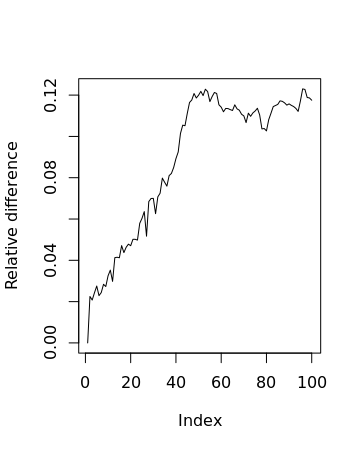
\includegraphics[width=0.33\textwidth]{wdbc_RD.png}}
	\subfloat[Waveform]{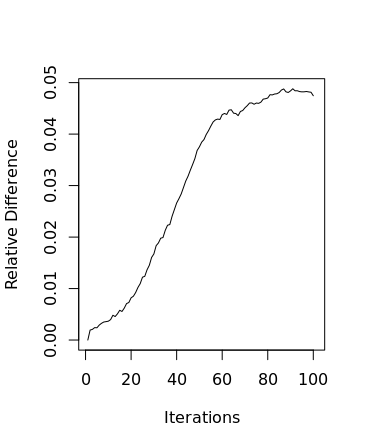
\includegraphics[width=0.33\textwidth]{waveform_RD2.png}}
	\subfloat[Spambase]{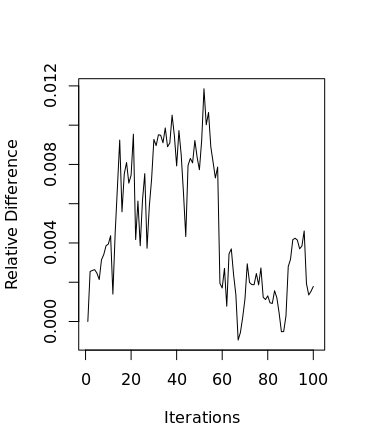
\includegraphics[width=0.33\textwidth]{spambase_RD3.png}}

    \centering
	\subfloat[Isolet]{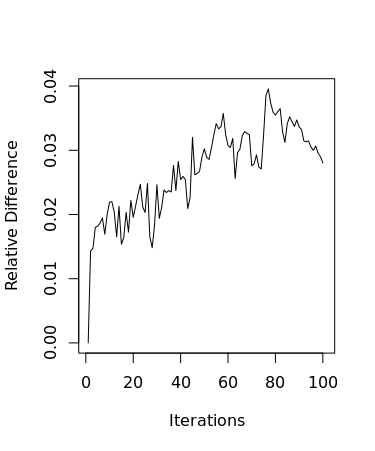
\includegraphics[width=0.33\textwidth]{isolet_RD2}}
	\subfloat[VHR Strasbourg]{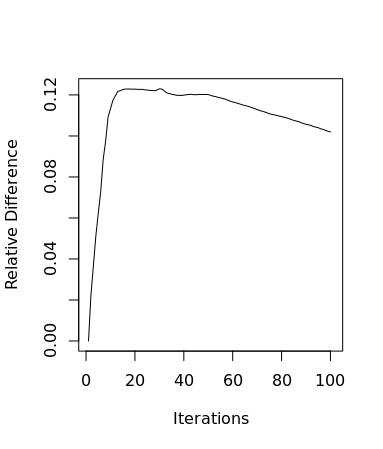
\includegraphics[width=0.33\textwidth]{vhr_RD}}
	\caption{Relative differences of the weighted criterion with and without $\beta$ optimization all along the learning process}
\label{fig:relative_difference}
\end{figure}

\subsection{Results}


\paragraph{Relative Difference of the criterion:}
The first experiment is about the evolution of the modified criterion presented in Eq.~\ref{eq:globalC2}. Figure~\ref{fig:relative_difference} shows the relative difference (RD) of this criterion between the original version of the collaborative SOM algorithm and our proposed version with the smart weights $\beta$. It appears that the relative difference between the criterion is always positive, meaning that the version with the $\beta$-weighting always improves the learning compared to the standard version. This can be understood knowing the interpretation in Sec.~\ref{sec:interpretation}: the algorithm tends to make views that agree with each others collaborate, so the $\beta$-weighting favors lower values of $C^j_i$ (better collaboration), improving the global criterion.

However, it also appears that all datasets are not treated equally by this method: the best mean RD goes from 0.4\% (Spambase) to 12\% (WDBC and VHR). Moreover, the gap size does not evolve the same way for all data bases: for WDBC, Waveform, Isolet and VHR Strasbourg, the gap is growing during several steps, while for Spambase, the evolution seems to stop quickly. We think that this phenomenon is partly caused by the information contained in each view: in some cases, a $\beta$-weighting will be useful because it will favor a collaboration that will greatly improve the global results, while in some other cases the results will approximately be the same than with the standard method, and therefore the RD is caped more quickly.

\paragraph{$\beta$ analysis:}
Now considering $\beta$ coefficients themselves, Figure~\ref{fig:betas} presents the different $\beta$ values obtained at the end of the collaboration process for each dataset. Table~\ref{tab:minmax} gives their corresponding minimum and maximum values. To recall, the value $\beta^j_i$ can be read as ``how much does view $j$ exchanges with view $i$ compared to the others''. The values on the diagonal -which are of no importance- are fixed to 1 to make the comparison easier. The last row of each matrix corresponds to the collaboration between each view and the artificially added noisy view of each data set (except for Waveform, for which the two last views were already noisy). 


Several points can be mentioned concerning these images. First, as one can see collaborations with noisy views are mostly weak:  the method presented here tends to minimize the impact of the collaboration between a useful view and a noisy one. This is particularly clear for the WDBC and VHR datasets where all $\beta$ on the last row are below 1, while all other factors are at least around 1. Secondly, one can see that the strong collaborations are mostly symmetrical. To continue with the WDBC example, we got $\beta_1^3 \approx \beta_3^1 > 1$. However this phenomenon is not true for less strong collaborations: for WDBC and VHR, we got $\beta_1^2 \neq \beta_2^1$ and $\beta_2^3 \neq \beta_3^2$. It appears that the algorithm leads to the creation of subgroups of views: when two views tend to collaborate, their other $\beta$ are approximately identical. This property can be seen as the continuation of the interpretation given in Sec.~\ref{sec:interpretation}: our method will favor the collaboration between agreeing views, leading to the creation of subgroups of views which have the same common behavior towards views outside of their group.

\begin{figure}[!h]
	\centering
	\subfloat[WDBC]{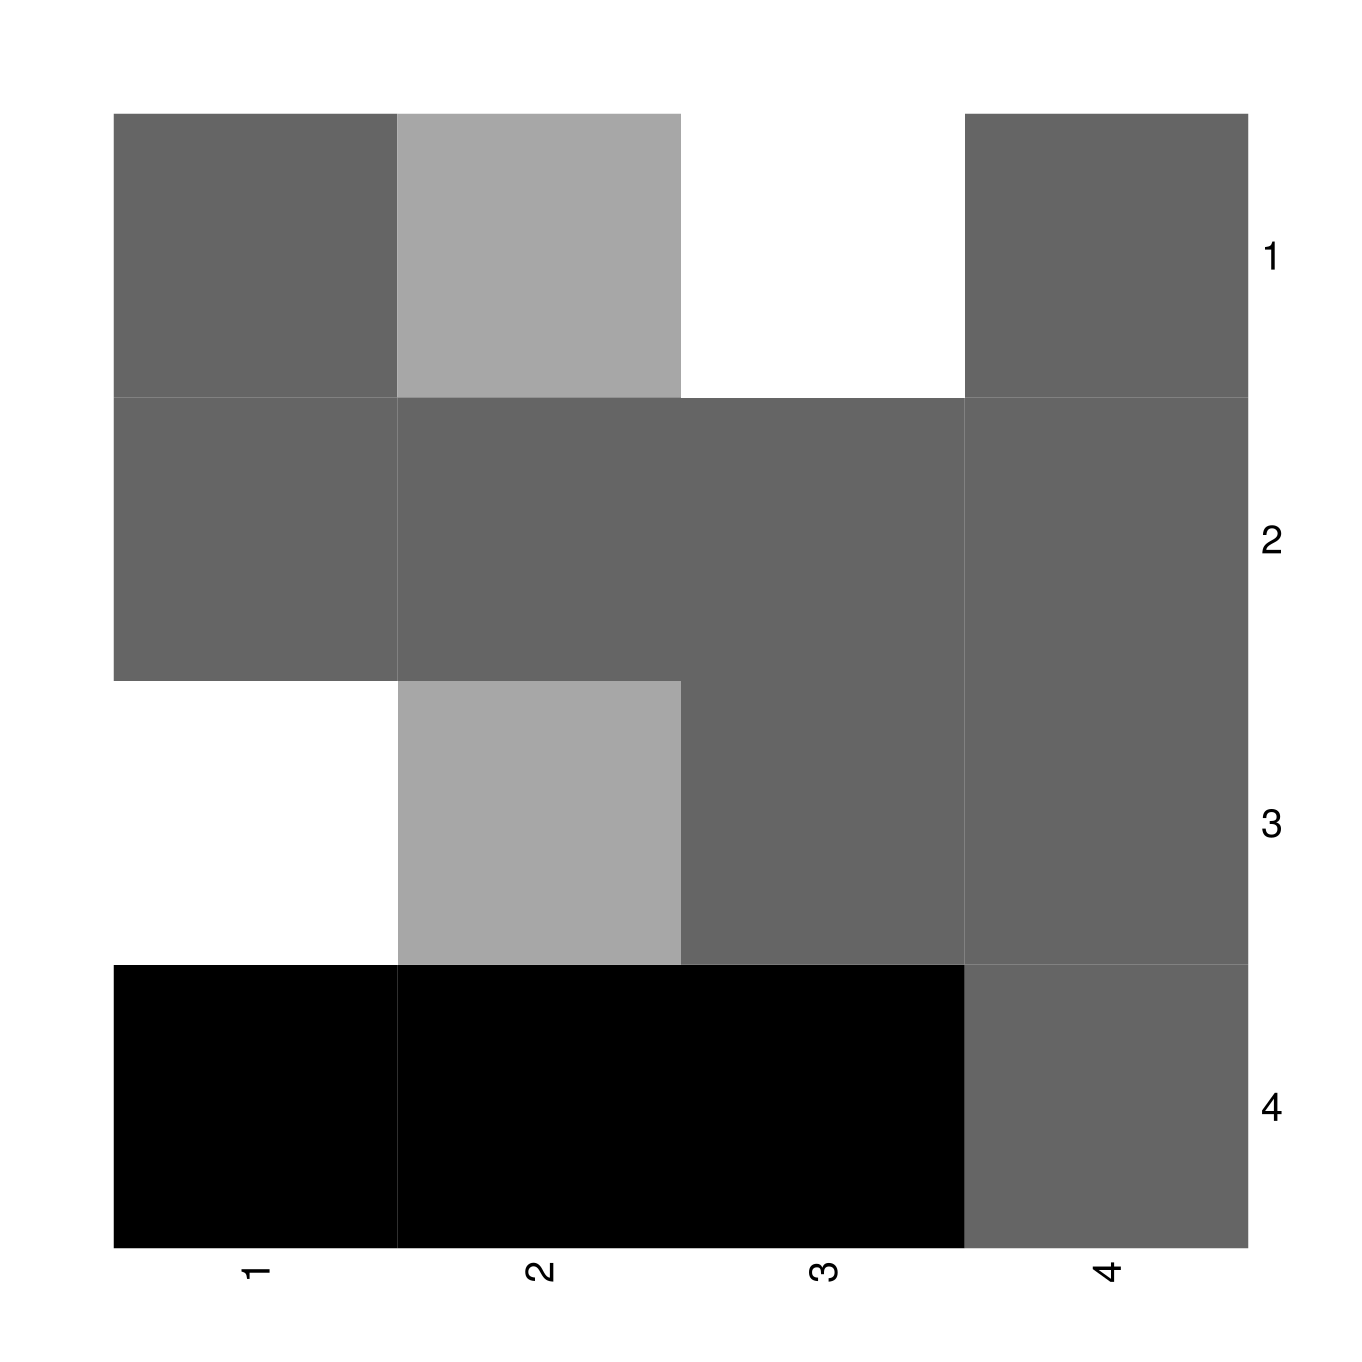
\includegraphics[width=0.33\textwidth]{wdbc_bw}}
	\subfloat[Waveform]{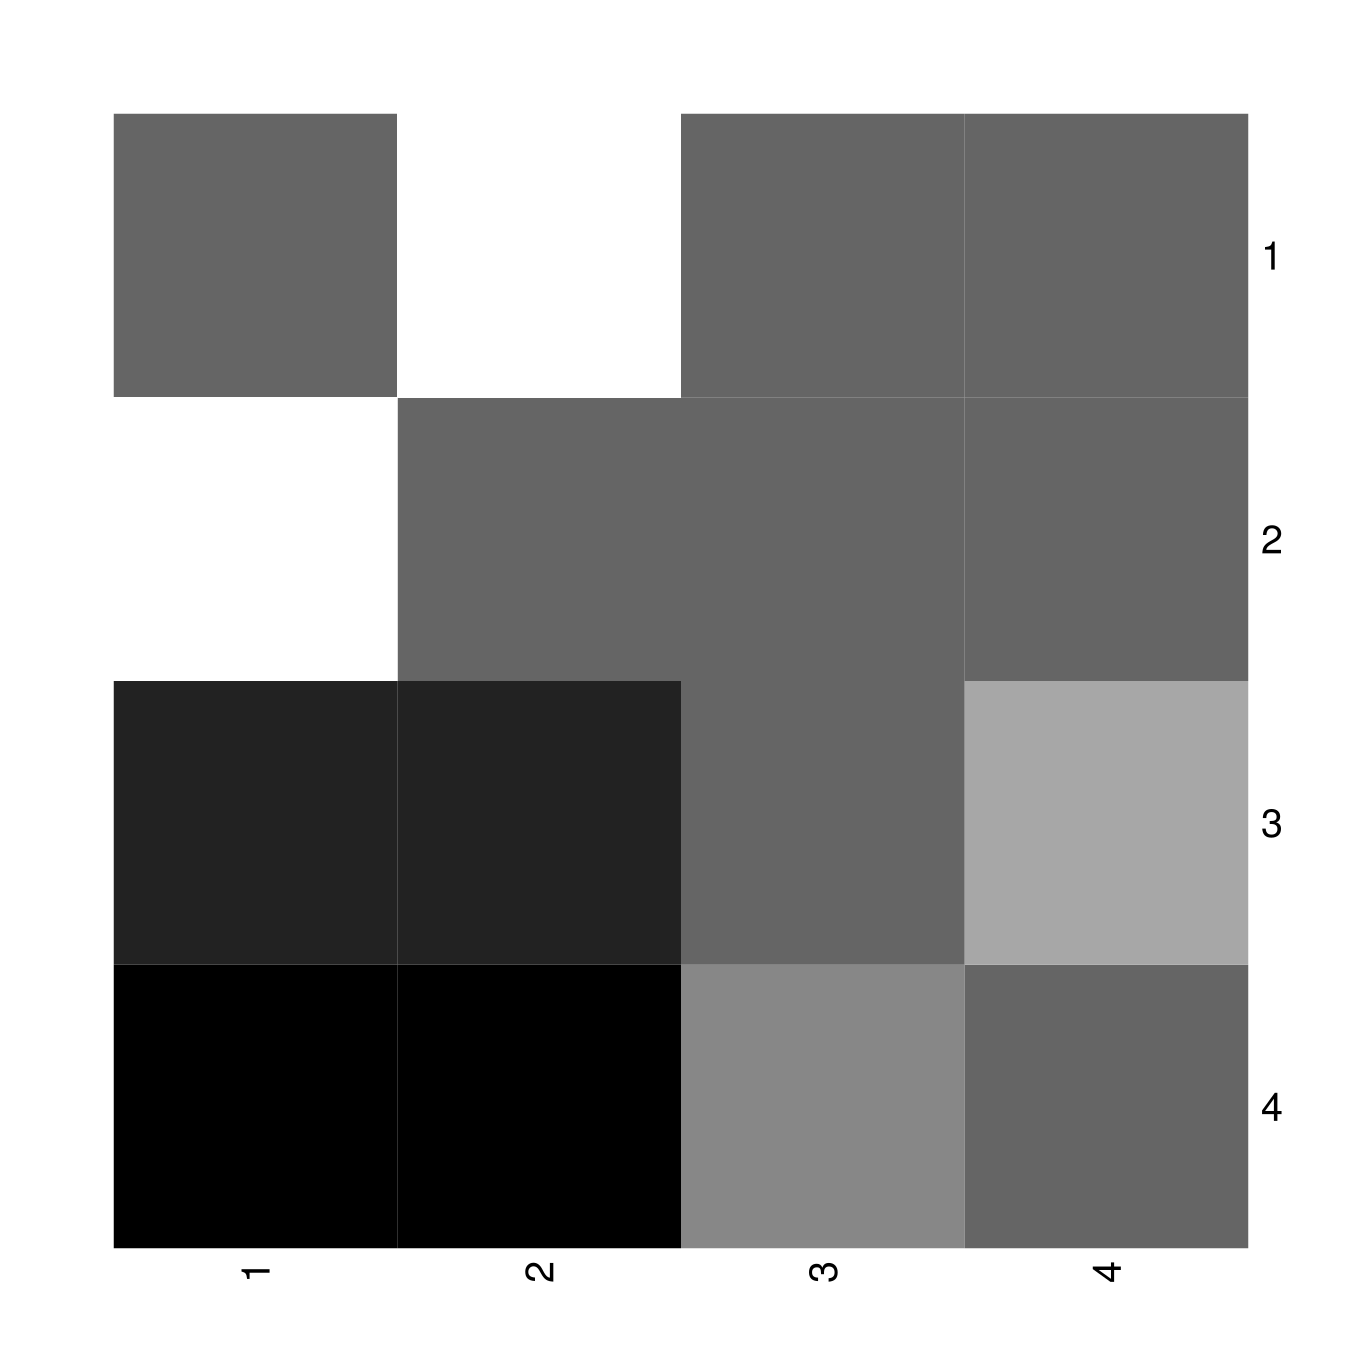
\includegraphics[width=0.33\textwidth]{waveform_bw}}
	\subfloat[Spambase]{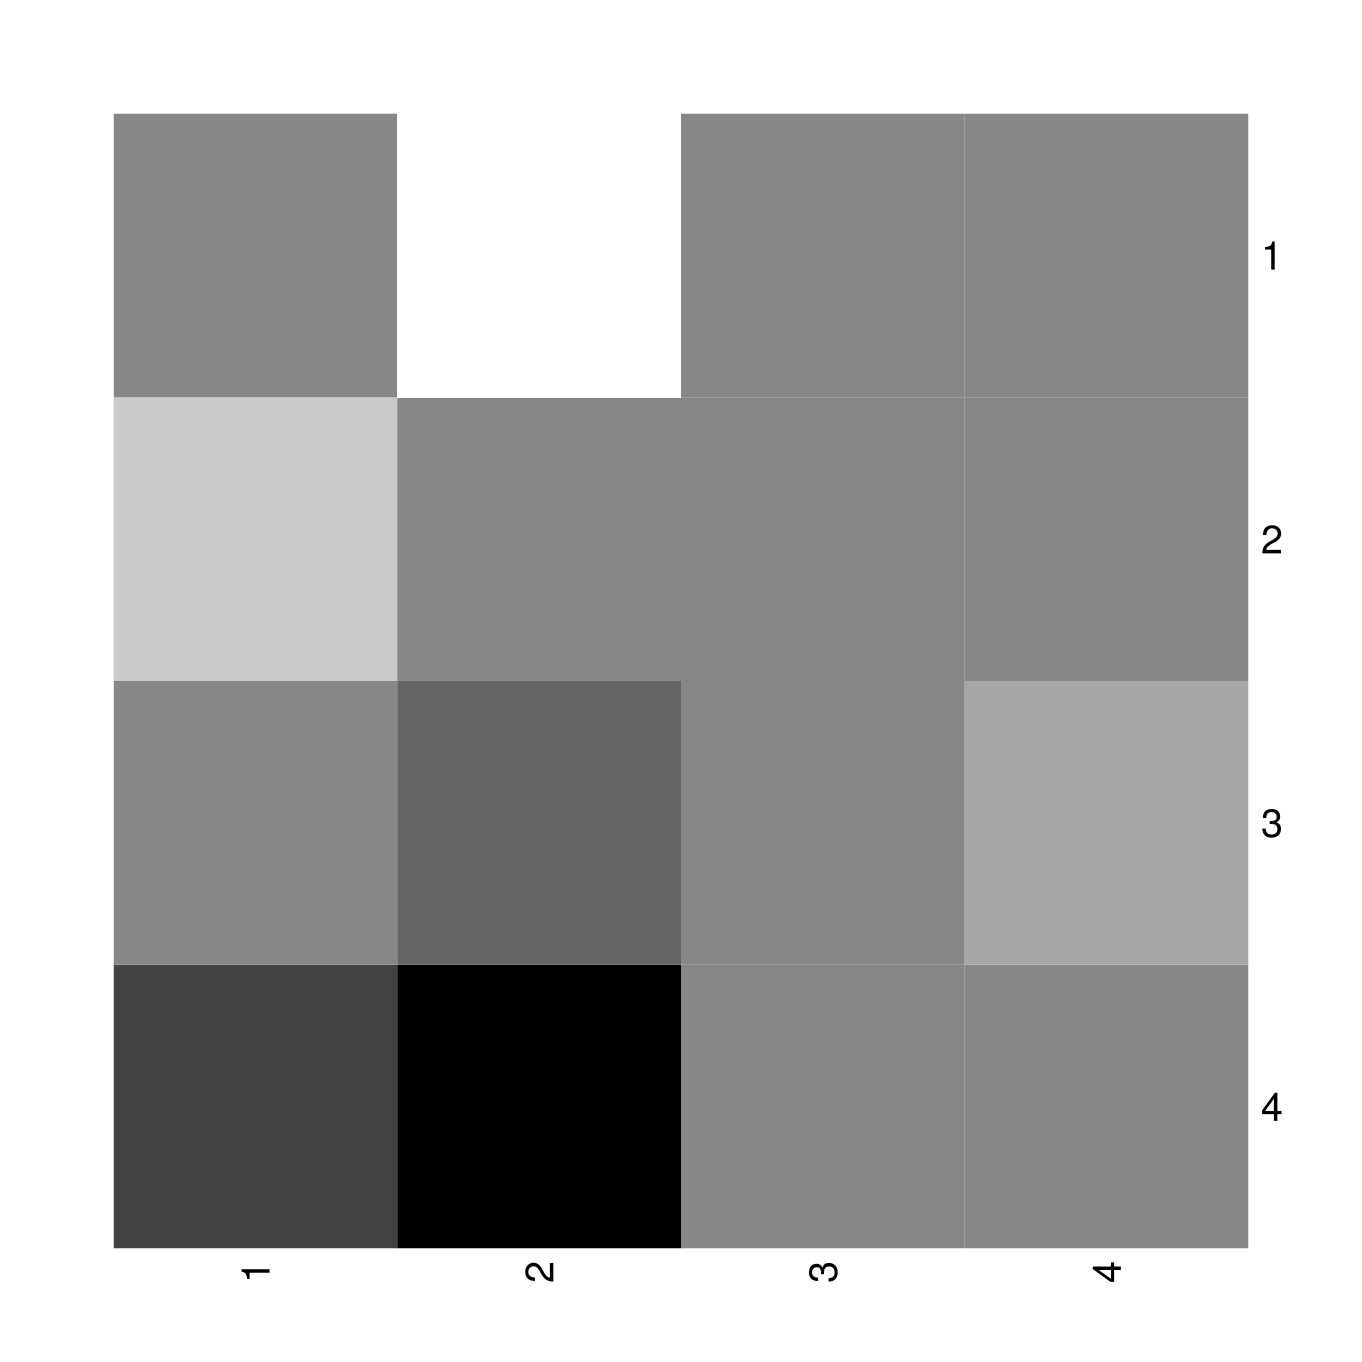
\includegraphics[width=0.33\textwidth]{spambase_bw}}

    \centering
	\subfloat[Isolet]{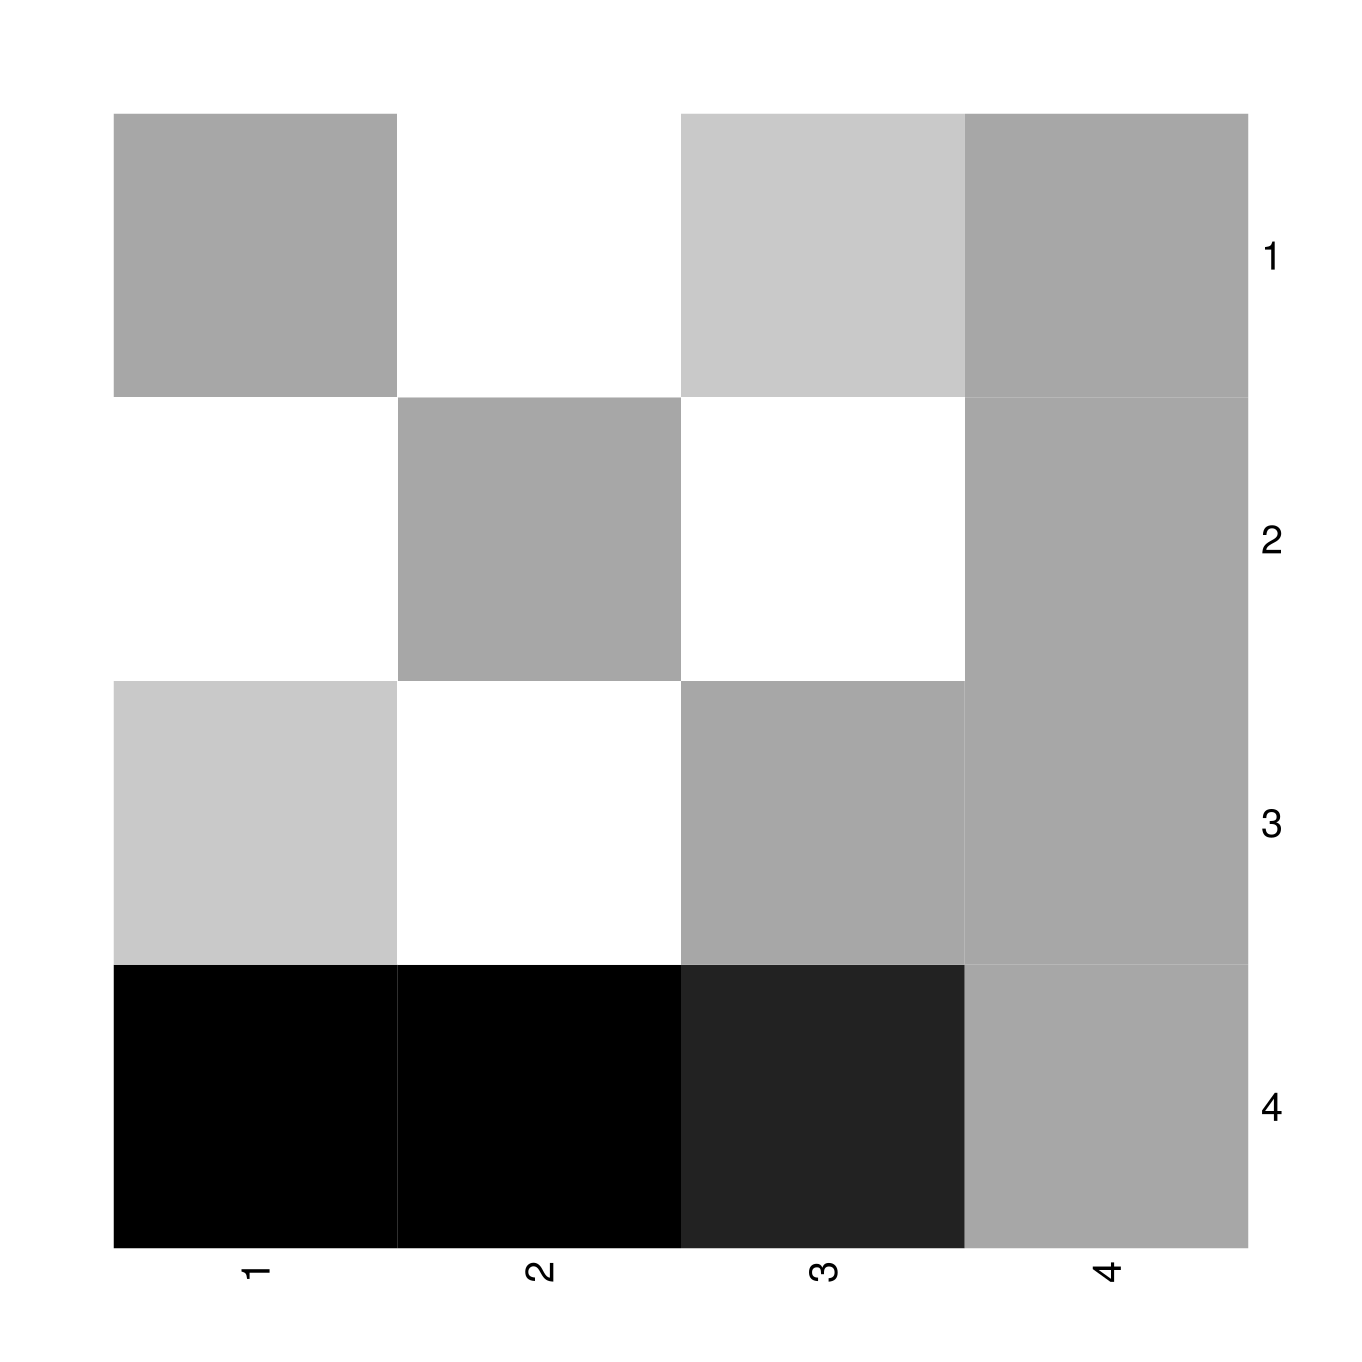
\includegraphics[width=0.33\textwidth]{isolet_bw}}
	\subfloat[VHR Strasbourg]{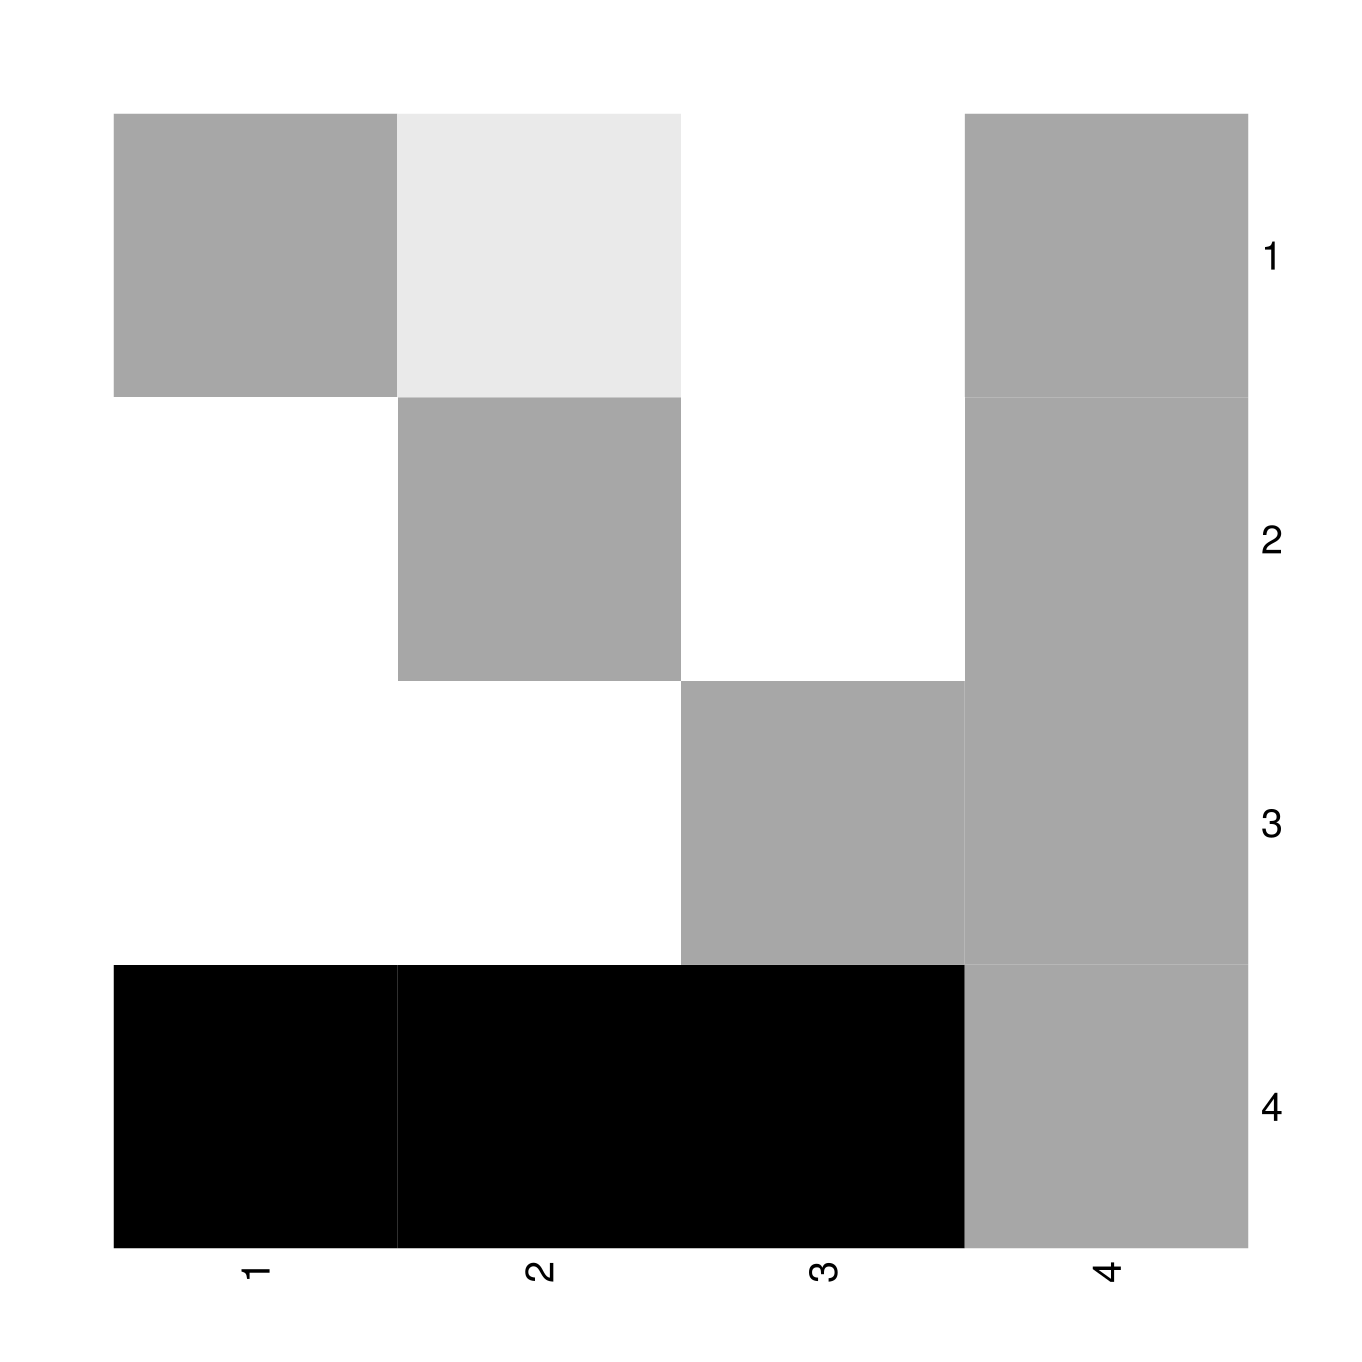
\includegraphics[width=0.33\textwidth]{vhr_bw}}
	\caption{Heatmap of the $\beta$ matrices for each dataset. Colors go from white (strong collaboration) to black (weak collaboration). The gray color on the diagonal stands for $\beta=1$.}
\label{fig:betas}
\end{figure}

\begin{table}[htbp]
	\caption{Minimum and Maximum values of $\beta$ got for each dataset.}
\label{tab:minmax}
	\begin{center}
		\begin{tabular}{cccc}
			\toprule
			Dataset & Minimum & Maximum & Difference
			\\
			\midrule
			WDBC & 0.51 & 2.04 & 1.53\\
			Waveform & 0.75 & 1.79 & 1.04\\
			Spambase & 0.77 & 1.37 & 0.60\\
			Isolet & 0.67 & 1.48 & 0.81\\
			VHR Strasbourg & 0.48 & 1.63 & 1.15\\
			\bottomrule
		\end{tabular}
	\end{center}
\end{table}

\paragraph{Purity and QE analysis:}
The last experiment consisted in the analysis of two criterion commonly found in 
the Kohonen's map literature, namely the purity and the quantization error. This 
analysis has been conducted in order to make sure that the collaborative phase 
and the $\beta$ weighting did not damage the final result of the learning.  
Table~\ref{tab:criterion} displays the mean values of each criterion for all the 
views, except the added noisy one. The results shows that our proposed weighting 
method, while succesful with unsupervised indexes has little to no impact on 
supervised criterions such as purity or quantization error. This result was to 
be expected since our proposed optimization does not bring any extra supervision 
compared to the original one, and it is therefore good already that it does not 
negatively impact supervised results.

\begin{table}[!h]
	\caption{Experimental results on different datasets}
\label{tab:criterion}
	\begin{center}
				\begin{tabular}{cccc}
			\toprule
			Dataset 	& Method 			& Mean Purity  & $qe$
			\\ 			\midrule
						Wdbc		& standard  		& 86.86 & 4.01  \\
						& $\beta$-weighting  	& 88.09 & 3.97  \\ \midrule 
			Isolet 		& standard    		& 55.37 & 125.32 \\
						& $\beta$-weighting    & 54.98 & 125.2 \\ \midrule 
			Waveform    & standard     		& 64.27 & 6.15  \\
						& $\beta$-weighting    & 65.40 & 6.16  \\ \midrule 
			SpamBase    & standard     		& 80.34 & 14.56 \\ 
						& $\beta$-weighting    & 80.24 & 14.54 \\ \midrule
			VHR Strasbourg    & standard     		& 48.94 & 3.37 \\ 
						& $\beta$-weighting    & 48.93 & 3.38 \\ \bottomrule
		\end{tabular}
	\end{center}
\end{table}




\section{Conclusion}
\label{sec:cc-conlu}

In this chapter, we have presented an optimization method for the case of horizontal collaborative clustering between SOM algorithms. Our method answers several questions regarding the tuning of the collaborative parameters between local and collaborative terms when using topological based collaborative clustering methods. Furthermore, we have also demonstrated how it can be used to make groups of similar maps, and to detect and discard noisy views.

Using our optimization model we have also found interesting properties, and in particular we have shown how diversity can be used to avoid bad influences from noisy or low quality view, and ultimately to improve the results of unsupervised collaborative learning. The conclusion from the theoretical part of this chapter is that a lower diversity is a good criterion to choose collaborators because it tends to favor stable solutions, which is a good thing since stability is a well known good quality criterion to find the intrinsic structures of the data set in unsupervised learning. However, one should keep in mind that the low diversity criterion has its limits and may hinder improvements in the collaborative process due to the lack of risk taking, or lead to no improvement at all if the diversity is too low. These later 2 issues are tackled in a paper where an alternative bandit optimization scheme is proposed for a similar collaborative clustering problem~\cite{Sublime2018a2}. 

Other possible extensions for this work could include similar studies on the case of vertical collaboration where the collaborating SOM algorithms handles different data sharing the same features, as well as the application of the same optimization technique for collaborative Generative Topographic Maps in a first time, and a further extension to non-topological collaborative methods in a second time.

The method presented in this chapter can be considered as an improvement of the inter-views collaboration using a traditional scalar weighting method. 

In the next chapter, we explore a collaboration method based on neural network and vectors rather than on scalar only. The complexity of this new method makes it possible to introduce a new use case to explore how an inter-view collaboration can be used to perform tasks different from clustering.
